\section{Objective and Sub-Tasks}
\label{sec:objective}
The main objective of this work is the development of a radar-based odometry system that estimates the vehicle ego-mmotion using mmWave radar sensors mounted at the fron of the vehicle setup in combination with an IMU for rotation compensation.
That motivation behind this approach is to explore radar as a cost-effective and robust alternative to the existing solutions based in vision or LiDAR-based odometry, particularly in conditions where those have the tendency to fail.
This builds on prior evidence that radar can support instantaneous ego-motion estimation through Doppler velocity cues \cite{EgoMotion_DopplerRadar}.

The system processes radar point cloud data enriched with range, angle, and most importantly Doppler velocity, to extract accurate motion estimates for ego-velocity or speed.
This enables the reconstruction of the vehicle’s trajectory and provides valuable input for SLAM applications.

\begin{figure}[!htbp]
    \centering
    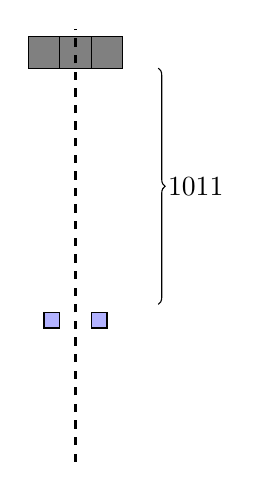
\begin{tikzpicture}
        \gokart{0}{0}{0}
    
        % Wall (three cubes)
        \draw[fill=gray] (-0.6,3) rectangle (-0.2,3.4);
        \draw[fill=gray] (-0.2,3) rectangle (0.2,3.4);
        \draw[fill=gray] (0.2,3) rectangle (0.6,3.4);
    
        % Dashed line from go-kart to wall (center axis)
        \draw[dashed, thick] (0,-2) -- (0,3.5);
    
        % Range brace annotation
        \draw [decorate, decoration = {brace, raise=10pt}] (0.7,3) -- (0.7, 0) node[pos=0.5,right=10pt,black]{\SIrange{10}{11}{\meter}};

        % Enlarged Radar sensor boxes
        \draw[fill=blue!30] (-0.4,-0.3) rectangle (-0.2,-0.1);

        \draw[fill=blue!30] (0.2,-0.3) rectangle (0.4,-0.1);
    \end{tikzpicture}
    \caption{Test scenario with dual front-mounted mmWave radar sensors.}
    \label{fig:test_scenario}
\end{figure}

The experimental setup is illustrated in Figure \ref{fig:test_scenario}, where two mmWave radar sensors are mounted at the front of a vehicle, providing overlapping fields of view to enhance environmental perception.
The dual-sensor configuration improves spatial coverage, reduces blind spots, and increases point density, resulting in more stable odometry processing compared to a single-sensor setup—an approach that aligns with multimodal methods for robust state estimation \cite{Multimodal_Offroad,HighSpeed_Estimation}.

By combining data from both sensors, including radial speed measurements derived from the Doppler effect, with the inertial measurement unit (IMU) for rotation compensation, the proposed system aims to ensure resilient odometry performance even under high-speed or degraded environmental conditions, where LiDAR-based odometry may fail \cite{HighSpeed_Estimation}.

Each radar perspective is processed independently and then merged into a single point cloud for further analysis.
This integration provides a more robust and reliable input to the odometry estimation pipeline, enabling the evaluation of radar-based odometry performance in realistic driving scenarios.

\subsection{Sub-Tasks}

The research objective, together with the constraints of using a dual-radar sensor, implied several practical sub-tasks:  
\begin{itemize}
    \item Designing a modular pipeline to acquire and decode synchronized radar data from both sensors.
    \item Investigating suitable sensor configurations to balance field of view, chirp bandwidth, update rate, and detection density.  
    \item Developing suitable mechanical mounts and selecting optimal sensor placement to ensure stability and maximize coverage.
    \item Applying RANSAC filtering on Doppler velocities to reject dynamic points and outliers.
    \item Implementing clustering methods to structure radar detections and isolate relevant features.  
    \item Optimizing the raw radar point cloud using additional information provided by the sensor itself (e.g., SNR, RCS, or range validity) to improve reliability before odometry processing.  
    \item Integrating Doppler velocity information into the odometry estimation process.   
    \item Employing submap aggregation to mitigate sparsity and improve stability. 
    \item Performing ICP alignment between submaps aggregated from both sensors to mitigate sparsity and noise. 
    \item Evaluating the influence of the dual-sensor arrangement on odometry accuracy and robustness. 
    \item Validating the complete system on real-world driving scenarios. 
\end{itemize}

As each sub-task builds upon the results of the previous one, the work followed an iterative and modular development approach, enabling gradual integration and continuous evaluation of the proposed system.  
The following sections detail the implementation and evaluation of each sub-task, culminating in a comprehensive radar-based odometry solution.